% !TeX spellcheck = en_US
\documentclass{article}
\usepackage{graphicx}
\usepackage{fancybox}
\usepackage{tikz}
\usepackage{algorithm}
\usepackage{amsmath}
\usepackage{algorithmicx}
\usepackage{algpseudocode}
\usepackage{graphicx}
\usepackage{caption}

\captionsetup{labelfont={color=black,bf}}

\makeatletter
\def\BState{\State\hskip-\ALG@thistlm}
\makeatother

\algdef{SE}[DOWHILE]{Do}{doWhile}{\algorithmicdo}[1]{\algorithmicwhile\ #1}%

\title{Homework 02: Binary Heaps}
\date{\today}
\author{Roberto Corti}

\begin{document}
	\maketitle
	
	\section*{Exercise 1}
	\textbf{Implement the array-based representation of binary heap together with the functions $\mathtt{HEAP MIN}$, $\mathtt{REMOVE ~ MIN}$, $\mathtt{HEAPIFY}$, $\mathtt{BUILD ~  HEAP}$, $\mathtt{DECREASE ~ KEY}$ and $\mathtt{INSERT ~ VALUE}$}. \\
	
	\noindent The array-based representation of a binary heap is implemented in the file \texttt{src/binheap.c}.  \\
	First of all I defined \texttt{total\_order\_type} in order to make an object able to express an ordering criterion inside the heap. Then, I create a struct \texttt{binheap\_type} in which it is stored:
	\begin{itemize}
		\item \texttt{A}: a void pointer that points array used to store heaps nodes.
		\item \texttt{num\_of\_elem}: a variable used to store the number of nodes.
		\item \texttt{max\_size}: a variable used to store the maximum number of nodes.
		\item \texttt{key\_size}: a variable used to store the size of the data type of the node.
		\item \texttt{leq}: a \texttt{total\_order\_type} for the ordering criterion of the heap.
		\item \texttt{max\_order\_value}: a variable used to store the maximum value for a node.
	\end{itemize}
Once defined this \texttt{struct}, the above requested functions are all implemented in \texttt{src/binheap.c}.
		
	\section*{Exercise 2}
	\textbf{Implement an iterative version of $\mathtt{HEAPIFY}$.} \\
	
	\noindent An iterative version of \texttt{HEAPIFY} has been implemented in \texttt{binheap.c}. The algorithm follows this pseudo-code:
	\newpage
	\begin{algorithm}
		\caption{\texttt{HEAPIFY(node)}}\label{euclid}
	\begin{algorithmic}
		\State $\textit{destination\_node} \gets \textit{node}$
		\Do
		
		\State $\textit{node} \gets \textit{destination\_node}$
		\State $\textit{child} \gets \text{RIGHT CHILD}(\textit{node})$
		
		\If{ $\text{ADDR}(\textit{node}) \preceq \text{ADDR}(\textit{child})$ } 
		\State $\textit{destination\_node} \gets \textit{child}$
		\EndIf
		
		\State $\textit{child} \gets \text{LEFT CHILD}(\textit{node})$
		
		\If{ $\text{ADDR}(\textit{node}) \preceq \text{ADDR}(\textit{child})$ } 
		\State $\textit{destination\_node} \gets \textit{child}$
		\EndIf
		
		\If {$\textit{destination\_node} \neq \textit{node}$}
		\State $\text{SWAP}(\textit{destination\_node}, \textit{node})$
		\EndIf
		
		\doWhile{$\textit{destination\_node} \neq \textit{node}$} % <--- use \doWhile for the "while" at the end
	\end{algorithmic}
	\end{algorithm}
	
	\section*{Exercise 3}
	\textbf{Test the implementation on a set of instances of the problem and evaluate the execution time.} \\
	
	\noindent In order to test the implementation I create two test codes: \texttt{src/test\_insert.c}, \texttt{src/heap\_test.c}. The first code performs a benchmark on the \texttt{insert\_key} function by increasing the size inserting nodes progressively. The asymptotic behaviour of this function is represented by the following plot.
	\begin{figure}[h]
		\centering
		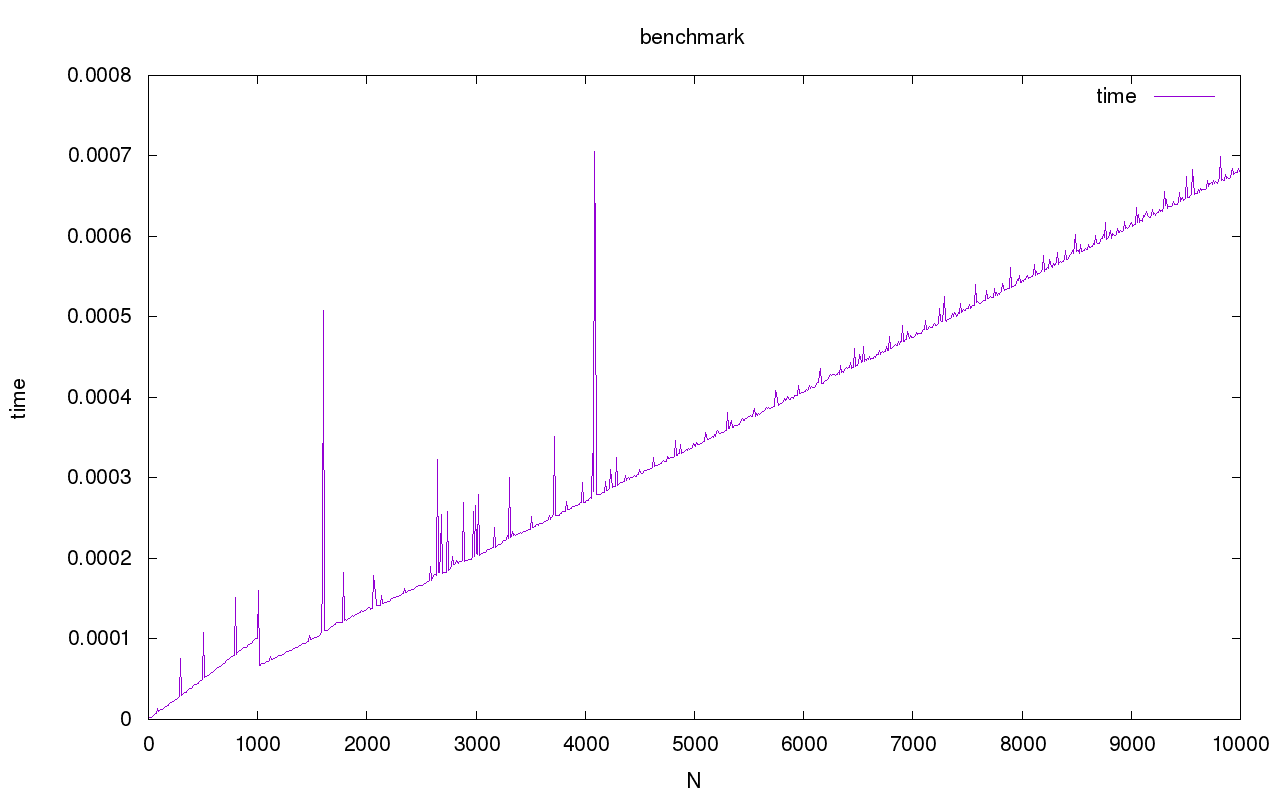
\includegraphics[width=0.8\textwidth]{../plot/plot_benchmark.png}  
		\caption{Benchmark of the \texttt{insert\_key} function.}
		\label{plot}
	\end{figure}
	\newpage
	\noindent On the other hand, \texttt{heap\_test.c} does a check of all the implemented functions just performing all of them written down \texttt{src/binheap.c}
	
	\section*{Exercise 4}
	\textbf{Show that, with the array representation, the leaves of a
	binary heap containing n nodes are indexed by $\lceil n/2 \rceil + 1, \lceil n/2 \rceil + 2, . . . n$.} \\



	\noindent If we consider the node at the index $ \lceil n/2 \rceil +1$ and by definition its left child will be at the index 
	$$ 
	\mathtt{LEFT}( \lceil n/2 \rceil +1 ) = 2(\lceil n/2 \rceil +1) > 2(n/2 - 1) = n.
	$$
	The left child is in a position greater than $\mathtt{HEAP\_SIZE}$, so the node at index $\lceil n/2 \rceil + 1$ has no children. Moreover, since a binary heap is a complete tree up to the leaf level, we conclude that the node $ \lceil n/2 \rceil +1$ is a leaf.
	
	\section*{Exercise 5}
	\textbf{Show that the worst-case running time of $\mathtt{MAX\_HEAPIFY}$ on a heap of size n is $\Omega(\log_2 n)$.  (Hint: For a heap with n nodes, give node values that cause $\mathtt{MAX\_HEAPIFY}$ to be called recursively at every node on a simple path from the root down to a leaf).} \\
	
	\noindent Consider the following max-heap in which we would like to represent the worst-case scenario:
	$$
	A[1] = 1, ~ \textmd{and} ~~ A[i] = 0 ~~ \forall i \in {2,..., n}.
	$$
	Then, in order to conserve the heap property we have to apply $\mathtt{MAX\_HEAPIFY}$ for every level of the tree  for pushing the element of value 0 to the leftmost leaf. $\mathtt{MAX\_HEAPIFY}$ will be then called $\log_2n$ times, so its running time will be $\Theta (\log_2n)$. Thus, the worst case running time of $\mathtt{MAX\_HEAPIFY}$ is $\Omega(\log_2n)$.
	
	\section*{Exercise 6}
	\textbf{Show that there are at most $\lceil n/2^{h+1} \rceil$ nodes of height $h$ in any $n$-element binary heap.} \\
	
	\noindent We know that for any $n > 0$, the number of leaves of nearly complete binary tree is $ \lceil n/2 \rceil$. With this result we can prove the thesis by induction. 
	\begin{itemize}
		\item Consider the case $h=0$; the thesis is satisfied since the unique level of the tree will contain $ \lceil n/2 \rceil = \lceil n/2^{0+1} \rceil$.
		\item Consider the thesis true for $h-1$.
		\item Let $N_h$ the number of nodes at leaf level of the tree $T_h$ that has height $h$. Consider the tree $T_{h-1}$ which is composed by $T_h$ up to its leaves. This tree will have $n' = n- \lceil n/2 \rceil$ nodes. Thus, if we consider $N'_{h-1}$ as the number of nodes at level $h-1$, this will be equal to $N_h$. Then, by using the induction step we have 
		$$
		N'_{h-1} = N_{h} = \lceil n' / 2^h\rceil = \lceil \lceil n/2\rceil / 2^h\rceil \leq \lceil n / 2^{h+1}\rceil.
		$$ 
		which is our thesis.
	\end{itemize}

	
	
	
\end{document}
